\label{Chapter:Introduction:DL}

In order to be able to understand the chapters that will come later in this document, it is important to make a brief introduction of what \emph{Deep Learning}(DL) refers to. Deep learning is included in the field of Machine Learning, which is also included in the field of general Artificial Intelligence.

In Chapter \ref{Chapter:Intro:Rep:Learning}, an intuitive definition of what Machine Learning is was given. We said that ML studies the algorithms that improve from experience. Tom M. Mitchell \citep{mitchell_machine_1997} provided a more formal definition of what \emph{learning from experience} means:

\begin{ndefC}
A computer program is said to \emph{learn} from experience $E$ with respect some class of tasks $T$ and performance measure $P$, if its performance at tasks in $T$, as measured by $P$, improves with experience $E$.
\end{ndefC}

We would also like to have a formal definition for deep learning. In \cite{deng_deep_2014}, multiple similar definitions are given. We present here the simplest of them:

\begin{ndefC}
\emph{Deep Learning} is a class of ML learning techniques that exploit many layers of non-linear information processing for supervised or unsupervised feature extraction and transformation, and for pattern analysis and classification.
\end{ndefC}

Usually, these techniques are based on the biologically inspired \emph{neural networks}(NNs), which consists of several connected units: the \emph{neurons}. Each neuron is basically a Perceptron, which is a is a weighted sum followed by a non-linear function, called an \emph{activator} in the ML context. Formally, the output of each neuron is 
\[
y = \phi\left(w_0 +\sum_{i = 1}^N w_i x_i \right) .   
\]
There are many activation functions, but the following examples must be remarked:
\begin{itemize}
\item Sigmoid. The sigmoid function is defined as follows:
\[
\phi(x) = \frac{1}{1+ e^{-x}}.
\]
This is one of the most common used activation functions. It is differentiable, monotonic and smooth. One of its main disadvantages is that at the right part of the function, the change in the values that the function takes converges to zero, so we get to the \emph{vanishing gradient} problem and the learning is minimal.

\begin{figure}[H]
    \centering
    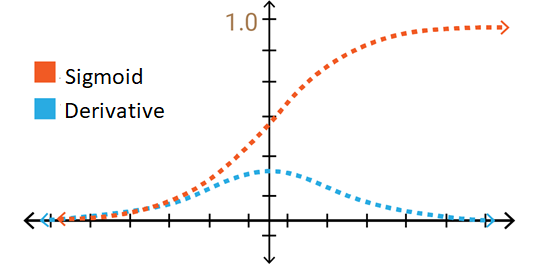
\includegraphics[width=0.5\linewidth]{sigmoid}
    \caption{Sigmoid. Image from \href{https://xzz201920.medium.com/activation-functions-linear-non-linear-in-deep-learning-relu-sigmoid-softmax-swish-leaky-relu-a6333be712ea}{this Medium article}. } \label{fig:sigmoid}
\end{figure}

\item Hyperbolic Tangent. This function is defined as follows:
\[
\phi(x) = \operatorname{tanh}(x) =  \frac{e^x - e^{-x}}{e^x + e^{-x}}.    
\]
This activation function has a small advantage over the sigmoid: its derivative is more steep, which means it can get larger values and the learning can be more efficient.

\begin{figure}[H]
    \centering
    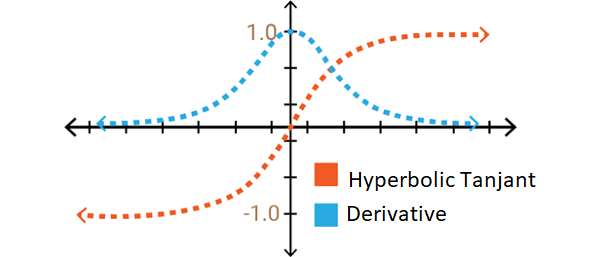
\includegraphics[width=0.6\linewidth]{tanh}
    \caption{Hyperbolic Tangent. Image from \href{https://xzz201920.medium.com/activation-functions-linear-non-linear-in-deep-learning-relu-sigmoid-softmax-swish-leaky-relu-a6333be712ea}{this Medium article}. } \label{fig:tanh}
\end{figure}

\item Rectified Linear Unit (ReLU). This function takes the following form:
\[
\phi(x) = \max\left(0,x\right).    
\]
ReLu is highly computationally efficient and non-linear. Its main problem is that when the inputs approach zero or are negative, the network can not perform back propagation and can not learn.

\begin{figure}[H]
    \centering
    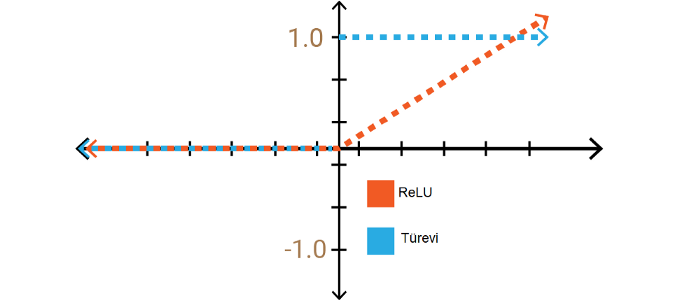
\includegraphics[width=0.6\linewidth]{relu}
    \caption{ReLU. Image from \href{https://xzz201920.medium.com/activation-functions-linear-non-linear-in-deep-learning-relu-sigmoid-softmax-swish-leaky-relu-a6333be712ea}{this Medium article}. } \label{fig:relu}
\end{figure}
\end{itemize}



\subsection{Neural Networks}

Using neurons and activation functions, we can formally define neural networks(NNs). A NN with $L$ hidden layers is a deterministic non-linear function $f$, parametrized by a set of matrices $W = \{W_0,\cdots,W_L\}$ and non-linear activation functions $\{\phi_0,\cdots,\phi_L\}$. Given an input $x$, the output $y$ of the network is calculated as follows:
\[
h_0 = \phi_0\left(W_0^Tx\right), \cdots, h_l = \phi_l\left(W_l^T h_{l-1}\right),\cdots, y = \phi_L\left(W_L^T h_{L-1}\right).
\]
Having a NN, we consider it \emph{deep} when the number of hidden layers (and, consequently, the number of matrices) is considered high. 

Neural networks use loss functions, which define how well the output returned by the network matches the real output, reducing the learning problem to an optimization problem. The problem is finding $W^{\operatorname{opt}}$, such that
\[
W^{\operatorname{opt}}   = \argmin_{w} \sum_{n = 1}^N \ell(y_n, f_w(x_n)),
\]
where $\mathcal D = \{(x_n,y_n)\}$ is a dataset and $\ell$ is the loss function.

This problem is solved using a variant of \emph{stochastic gradient descent (SGD)}. This algorithm involves the computation of the loss function $l$ derivatives respect to the network parameters, and updates the parameters using this derivatives. Specifically, the parameters are updated as follows:
\[
W_{t+1} = W_t + \eta \nabla \ell(W_t),
\]
where $\eta \in \R^+$ is a small constant called the \emph{learning rate}. This algorithm guarantees convergence to local minimums of $f$ and, if $f$ is convex, the algorithm converges to a global minimum.

The last comment about neural networks is that, since the weights $W = \{W_0,\cdots,W_L\}$ are constantly updated, the derivatives have to be computed repeatedly. The computational cost of this is quite high. \emph{Backpropagation} was born to calculate the derivatives of the weights much faster. The intuitive idea is that the gradient of the layer $l$ is computed using the gradient of the layer $l+1$ using the chain rule.

Understanding both SGD and Backpropagation is crucial for understanding how NNs  work. However, in the experimentation part of this work we will focus on researching how a few hyperparameters affect the results of the proposed frameworks, so no further explanation on these important concepts will be provided.

\subsubsection*{Convolutional Neural Networks}

Convolutional Neural Networks (CNNs) are a specific type of Neural Networks. The difference that we have between CNNs and NNs is that CNNs assume that the inputs have local dependencies. For instance, using an image, a CNN assumes (most of the time correctly) that given a pixel $x_{ij}$ of an input $x$, the neighbours of this pixels will have similar values or intensities. This allows us to encode certain properties into the architecture of the network.

If we use colored images, the input of the CNNs are 3-dimensional volumes, which will be transformed in some layers to other 3-dimensional volumes. In order to do this we have different types of layers, remarking \emph{convolutional} layers, \emph{pooling} layers and \emph{fully connected} layers. The most important ones are convolutional layers.

Convolutional layers receive a \emph{tensor} with shape $k \times n \times m \times c$, which means that the layer receives $k \in \mathbb N$ inputs of sizes $n \times m \times c$.  After the convolutional layer, the input has shape $k \times n' \times m' \times c'$, where $n'$ can be different from $n$ (respectively $m',c'$). One convolutional layer can apply one or several filters to the same input, producing different 2-dimensional activation maps that are stacked along the depth dimension to produce the output.

Formally, a convolution is the process of adding each element of the image to its local neighbours, weighted by a kernel. That is in our case performing a dot product between the input and the filter. We obtain
\[
g(x,y) = \omega \star f(x,y) = \sum_{dx = -a}^a \sum_{dy = -b}^b \omega(dx,dy)f(x+dx,y+dy),    
\]
where $g(x,y)$ is the pixel $(x,y)$ of the filtered image, $f(x,y)$ is the same pixel in the original image, and $\omega$ is the filter kernel. Depending on the filter kernel, the result will be different. 
\begin{nexample}
If we want to produce noise reduction in an image, we use Gaussian Blur, which kernel is calculated by a Gaussian function like the one in Equation \eqref{gaussian:function}. For instance, a $3\times 3 $ gaussian kernel would approximately be:
\[
\frac{1}{16}\begin{bmatrix}
    1 & 2 & 1\\
    2 & 4 & 2\\
    1 & 2 & 1
\end{bmatrix}.
\]
\end{nexample}

\subsection{Siamese networks}


We have to remark an emerging kind of networks that have proved to be very useful in the representation learning task. We introduce them with the following definition.

\begin{ndefC}
A \emph{siamese neural network} \citep{voinov_explanation_2021} is a type of NN architecture that contains (typically) two NNs which have the same configuration, parameters and weights. The parameters are updated the same way across both networks. 
\end{ndefC}

\begin{figure}[H]
    \centering
    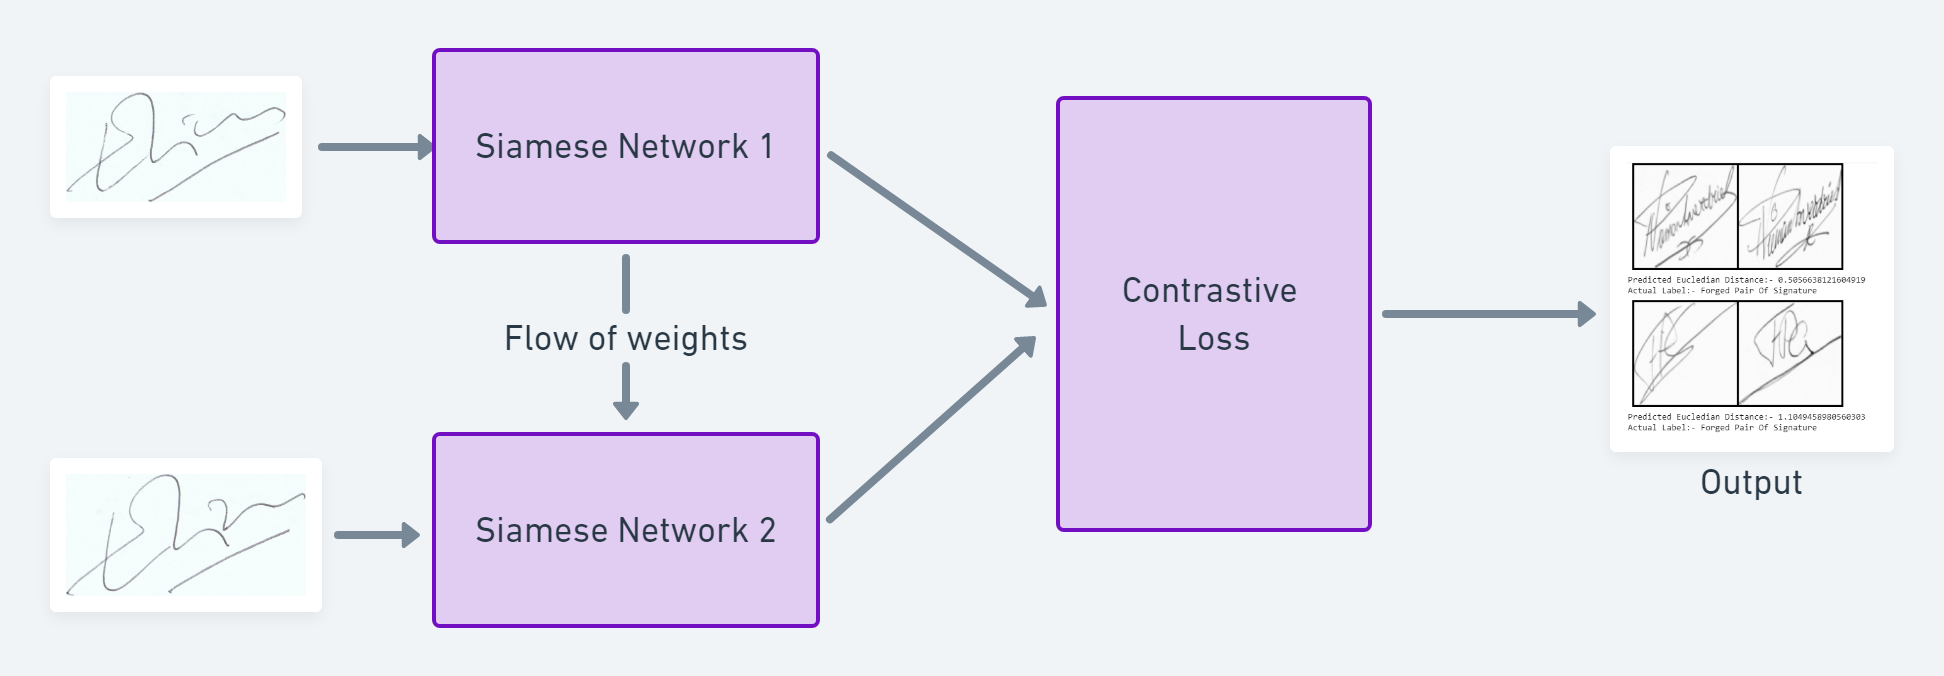
\includegraphics[width=0.8\linewidth]{siamese}
    \caption{Example of siamese network used for signature verification. Image from \href{https://towardsdatascience.com/a-friendly-introduction-to-siamese-networks-85ab17522942}{towards data science}. } \label{fig:resnet:block}
\end{figure}


These networks are usually used to find the similarity between the inputs by comparing produced feature vectors. They are more robust to class imbalance, nice to an ensemble with the best classifier (since the classifier is built on top of the representation extractors), and learn from semantic similarity. However, these architectures also have some drawbacks such as longer training times and that the output is not always a probability but distance between classes.




\subsection{ResNet}

To finish with this introduction to CNNs, we will present a widely used CNN architecture. Since CNNs appeared, people tried to build such deep networks that were very hard to train. When deeper networks start converging, a degradation problem ocurred: with the network depth increasing, accuracy gets saturated and then it degraded rapidly. \emph{ResNet} \citep{he2015deep} brought and end to this problem, allowing the training of very deep models with up to hundreds of layers.

In the paper, they mention that if $\mathcal H(x)$ is the underlying map of a sequence of layers and knowing that it can be asymptotically approximated, we can also approximate its residuals
\[
\mathcal F(x) = \mathcal H(x) - x.    
\]
Then, the original function becomes $\mathcal F(x) + x$. In order to achieve this, they introduced the \emph{Residual Block}, a block of layers that introduces skip or shortcut connections that makes it easy for networks to represent the identity mapping. We can see one of this blocks depicted in Figure \ref{fig:resnet:block}.

\begin{figure}[H]
    \centering
    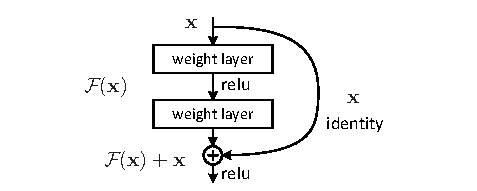
\includegraphics[width=0.6\linewidth]{block}
    \caption{Residual Block. Image from \cite{he2015deep} } \label{fig:resnet:block}
\end{figure}

Usually, ResNet comes accompanied by a number (e.g. \emph{Resnet-50}), that indicates the number of layers it has. Usually, a \emph{batch normalization} is used after each convolution and ReLU is used at the end of each group of layers.

% Please add the following required packages to your document preamble:
% \usepackage{multirow}
\begin{table}[H]
    \centering
    \begin{tabular}{|l|l|c|}
    \hline
    Layers                      & Output Size                     & Resnet 18                                                                     \\ \hline
    conv1                    & $112\times112$                  & $7 \times 7, \ 64$, stride 2                                                  \\ \hline
    \multirow{2}{*}{conv2} & \multirow{2}{*}{$56 \times 56$} & $3 \times 3$ max pool, stride 2                                               \\ \cline{3-3} 
                                &                                 & $\begin{bmatrix}3 \times 3 , & 64 \\ 3 \times 3,& 64 \end{bmatrix} \times 2$  \\ \hline
    conv3                  & $28 \times 28$                  & $\begin{bmatrix} 3\times 3, & 128 \\ 3\times 3, & 128 \end{bmatrix} \times 2$ \\ \hline
    conv4                  & $14 \times 14$                  & $\begin{bmatrix} 3\times 3, & 256\\ 3\times 3, & 256\end{bmatrix} \times 2$   \\ \hline
    conv5                  & $7 \times 7$                    & $\begin{bmatrix} 3\times 3, & 512\\ 3\times 3, & 512\end{bmatrix} \times 2$   \\ \hline
                                & $1\times 1 $                    & average pool, 1000-d fc, softmax                                              \\ \hline
    \multicolumn{2}{|c|}{Number of parameters}              & $11.400.000$                    \\ \hline

    \end{tabular}
    \caption{Resnet 18 architecture.}
    \label{arch:resnet:18}
    \end{table}

For instance, having a look at the Table \ref{arch:resnet:18}, in the convolution block \emph{conv2}, we have two convolutions with kernel size $3\times 3$ and depth size $64$. This would be one of the blocks, represented in Figure \ref{fig:resnet:block}. However, since at the right hand side of the matrix we have a $\times 2$, it means that we will have two of this blocks in this convolution group.

\subsection{Data augmentation}

In the general problem of performing a DL task, it may happen that the amount of data, either labeled or unlabeled, is not enough to give the model the number of examples that it needs to learn. 

\begin{ndef}
\emph{Data augmentation} are techniques used to increase the amount of data by adding modified copies of the already existing data or newly created synthetic data also from the existing one. 
\end{ndef}

In our self-supervised problem, data augmentation gains even more importance. It has been empirically shown that choosing the appropriate techniques and the order of the application of them to the images can cause a huge improvement on the results \citep{chen_simple_2020}.

Depending on the kind of data that we are facing, the techniques change. For instance, if we are working in the field of Natural Language Processing (NLP), which involves applying ML to texts, we should use techniques such as \emph{Back translation} or \emph{Synonym replacement}. If we try to process audio we can use \emph{Noise Injection} or changing the \emph{Speed} of the audio.

In our case, we will be working with images. Let us present some examples that can be used for data augmentation in the computer vision field.

\subsubsection*{Rotations and flips}

A very common data augmentation technique is the \emph{rotation} of the image a certain amount of degrees (usually one of the following: $\left\{\frac{\pi}{2}, \pi, \frac{3}{2}\pi\right\}$) using the center of the image as a rotation center. To do this, we only have to consider the following transformation:
\[
\begin{pmatrix} x' \\ y' \end{pmatrix} = \begin{pmatrix} \cos(\theta) & - \sin(\theta) \\ \sin(\theta) & \cos(\theta)\end{pmatrix} \begin{pmatrix} x \\ y\end{pmatrix}  ,  
\]
where $(x,y)$ is the pixel of the image that we will rotate and $\theta$ are the degrees that the image will be rotated.

This rotation can be composed (or not) with a \emph{flip} operation. That operation consists of applying a symmetry respect the central column of an image. Clearly, a flip can be applied on its own and it is still generating a new example.

\begin{figure}[H] 
    \centering
    \subfloat[Tulips]{%
        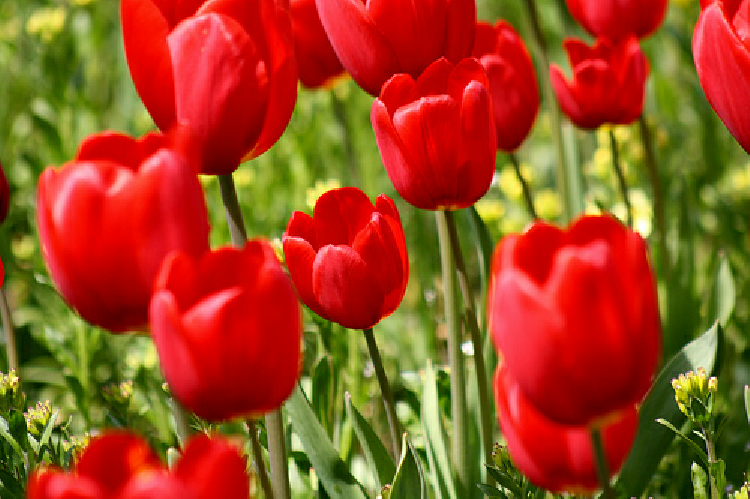
\includegraphics[width=0.45\textwidth]{tulips}%
        \label{fig:original:flowers}%
        }%
    \hfill%
    \subfloat[Rotated, flipped tulips]{%
        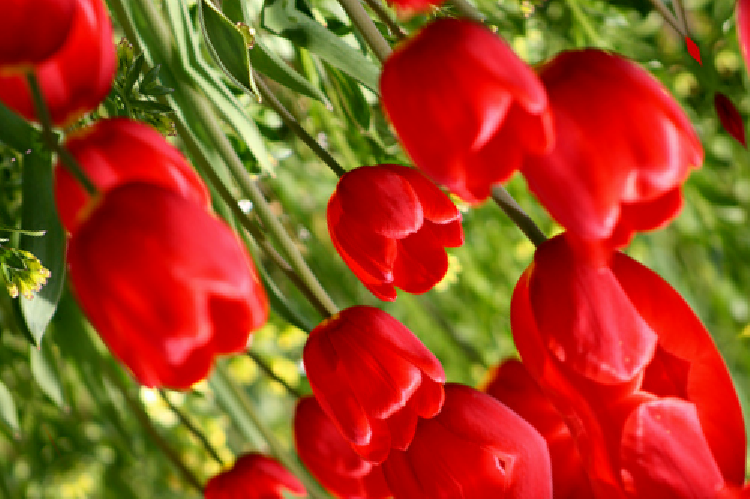
\includegraphics[width=0.45\textwidth]{tulips-rot1}%
        \label{fig:rot:flip:flowers}%
        }%
        \caption{The image on the left is the original image, and the image on the right is a new example generated by first a rotation of a random angle and then a flip.}
\end{figure}


\subsubsection*{Random crop with resize}

Another type of example generation is taking a crop randomly out of the image, making sure that the whole crop stays inside the image, and then resizing it back to the original image size. 

If an image is sized $n\times m$ with $n,m \in \mathbb N$, this method consists of selecting a rectangle of size $n'\times m'$ with $n' \leq n, m' \leq m$ of the original image and then resizing it back via upsampling\footnotemark.

%------------- Footnotemark
\footnotetext{Upsampling is increasing the size of an image by inserting new rows and columns in the image matrix and interpolating the values of the introduced pixels using the pixels that we already had in the image.}
%----------------------


\begin{figure}[H] 
    \centering
    \subfloat[Tulips]{%
        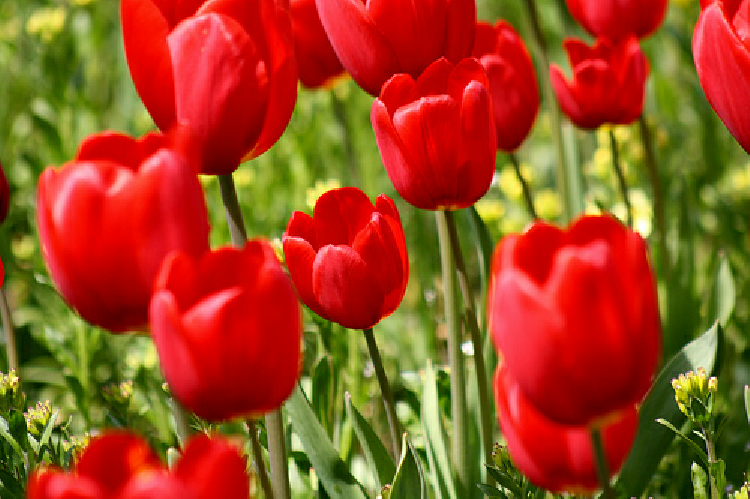
\includegraphics[width=0.45\textwidth]{tulips}%
        \label{fig:original:flowers:sidecrop}%
        }%
    \hfill%
    \subfloat[Random cropped, resized tulips]{%
        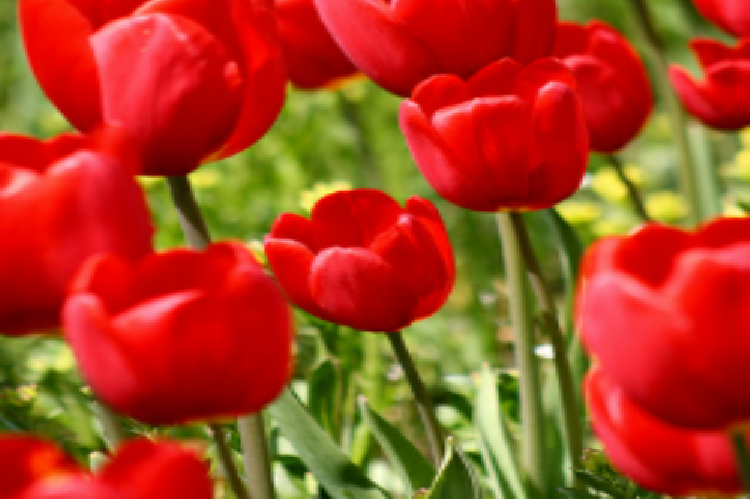
\includegraphics[width=0.45\textwidth]{tulips-randomcrop}%
        \label{fig:crop:resize:flowers}%
        }%
        \caption{The image on the left is the original image, and the image on the right is a new example generated by performing a random crop of the image and then resizing the crop to the original image size.}
\end{figure}

This can be useful to obtain images that are similar to each other, for instance, taking two crops of the same image. However, this could also lead to the model to learn an specific kind of data that is not relevant in general: the image data histogram. Let us see the image data histograms for both the original image and the random cropped image:

\begin{figure}[H] 
    \centering
    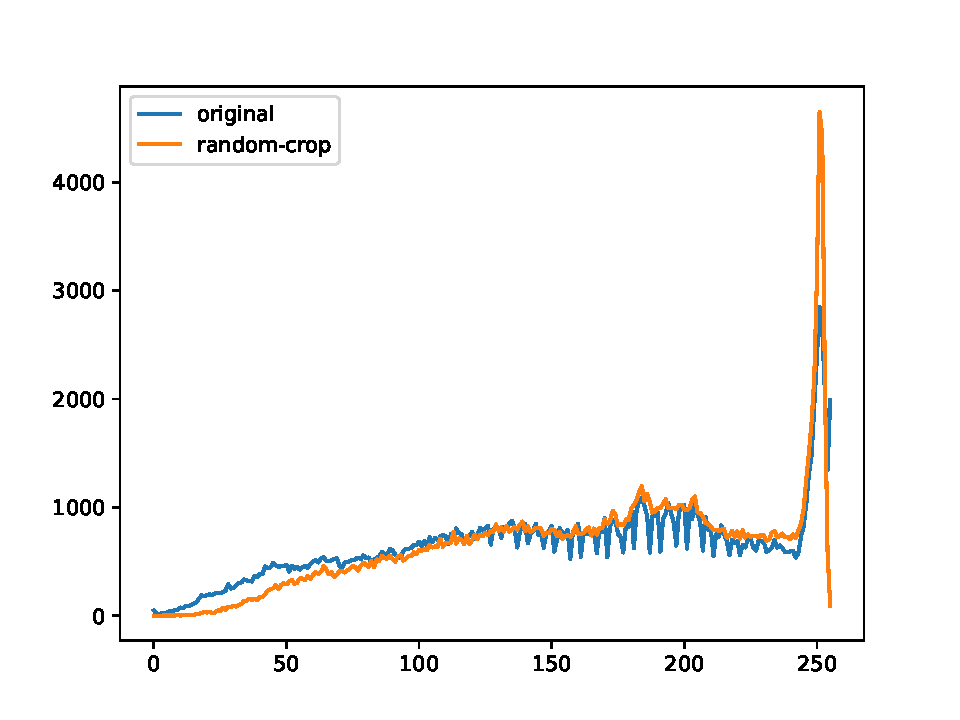
\includegraphics[width=0.6\textwidth]{tulips-histogram}%
        \label{fig:hist:orig:cropped}%
        \caption{Histogram for both the original image on blue and the random crop on orange.}
\end{figure}

As we can see, the histograms of both the images are quite similar, so a DL model could learn to identify similar objects making use only on this data histogram, which would not be very effective since the same object can have many different histograms. Because of this, this random crops are useful but the random cropped images have to be applied more functions in order to be really useful for the training of our models. 


\subsubsection*{Random color jitter}

This kind of data augmentation is not always used, but it is very interesting in our case. The random crops produced very similar data histograms since the colors in the original image and the cropped image are very similar. We can try to change this by randomly modifying the value of the pixels by changing the brightness, saturation or the contrast of the image.

\begin{figure}[H] 
    \centering
    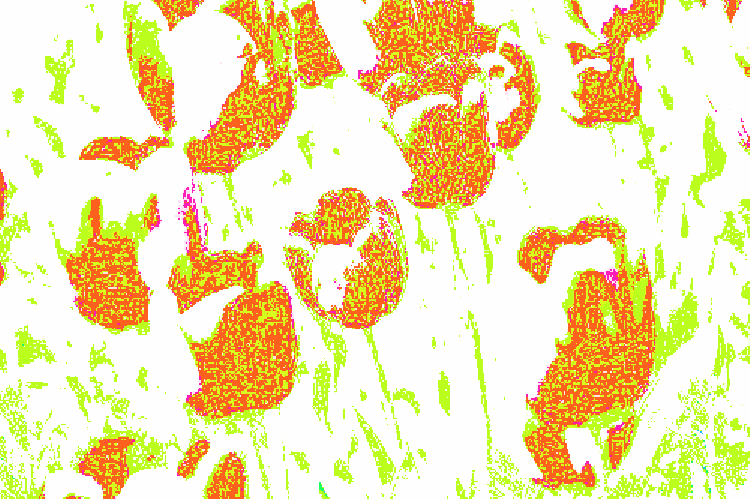
\includegraphics[width=0.5\textwidth]{tulips-colorjitter}%
        \label{fig:color:jitter}%
        \caption{Color jitter applied to tulips image.}
\end{figure}

We would like to see if there is a difference between the histograms of the cropped image compared with the color jittered image. The result is the following:

\begin{figure}[H] 
    \centering
    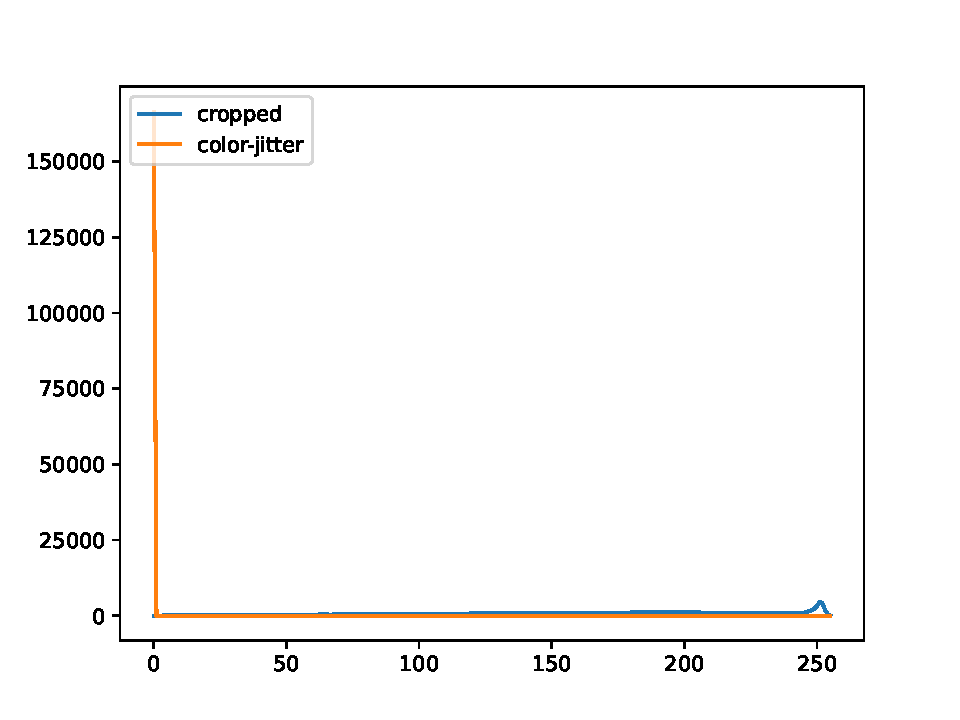
\includegraphics[width=0.5\textwidth]{histogram-croppedvsjitter}%
        \label{fig:color:jitter}%
        \caption{Histograms of the color jitter image in orange and cropped image in blue.}
\end{figure}

As we can see, since in the color jittered image most of the pixels turn white, the histograms get a big difference this time specially in the left side. This way, if we use both augmentation composed, we will avoid our model to learn only from the data histogram of our images.

